\chapter{Fish at river temperature: what the copy-error reading did and did not show}\label{ch:salmonid}
% Sources: PROC-SALMON-01, PROC-CHARR-01, PROC-RIMOUSKI-01 (pre-registrations and outcomes), DEV-COHO-CC-01 (note and outcome),
% and the per-fish tables salmon_readings.csv, charr_readings.csv, rimouski_readings.csv, coho_cc_fish.csv. Figure: figscripts/fig_p4_fish_library.py.

\section{Why fish, and what was asked}

Salmonids are the first animals other than humans that we read on single molecules. They answer two questions that human cells
cannot. First, an ectotherm's cells copy their methylation at the temperature of the water, not at 37~\textdegree C, so a fish
reading tests whether the holding energy of Chapter~\ref{ch:iama} is fixed in joules or fixed in units of $\kB T$
(Eq.~\eqref{eq:eps0T}, Chapter~\ref{ch:temperature}). Second, hatchery and wild fish of one river, or selected and control lines
reared side by side, ask whether the copy error is a property of the individual animal. Fish red blood cells are nucleated, so a
blood sample is close to one cell type and needs no separation step.

Four public data sets have been read with one statistic. Three were pre-registered with numerical bars before any read was
aligned; the fourth is a development reading whose checks were written down before any fish was scored. This chapter gives each
set, its bars and its outcome, and then the one lesson they share.

\section{The statistic, and the guard added after the first set}

The reading is the copy error of Eq.~\eqref{eq:eps}: on molecules with at least six CpG calls of which at least 80~\% are
methylated, an unmethylated interior CpG between two methylated neighbours is an isolated error, and $\varepsilon$ is the pooled
number of errors over opportunities for one fish. Three instrument terms are read from the same library and printed beside every
reading: the sequencing error $s$ (mismatches at bases bisulfite conversion cannot touch), subtracted to give
$\varepsilon_{\rm corr}=\varepsilon-s$; the conversion failure $c$, the methylated fraction of non-CpG cytosines; and, for
whole-genome libraries, the duplicate fraction. A CpG is masked for one fish when more than 30~\% of at least five qualifying
molecules carry an error there, since that is a C$\to$T variant rather than a copying error. The holding energy is
$E=\kB T\ln[(1-\varepsilon)/\varepsilon]$. Each set is also split into two halves (by run, or by alternate molecules) to test
whether the instrument repeats itself on one fish. \derived{} for the form of $E$; the selection rules are \calibrated.

The first set showed that the spread between fish can follow the library rather than the fish. From the second set on, every
pre-registration carries a guard: if the per-fish copy error correlates with conversion failure, duplicate fraction or masked
fraction at $|\rho|\ge0.30$ (Spearman), no difference between groups of fish is interpreted, whatever its $p$-value.

\section{Methow River steelhead: red cells and sperm (PROC-SALMON-01)}

\paragraph{Data.} Twenty adult male steelhead (\emph{Oncorhynchus mykiss}) returning to the Methow River in 2014, ten of hatchery
and ten of natural origin, each sampled for red blood cells and sperm~\cite{Gavery2018}. The libraries are reduced-representation
bisulfite sequencing with post-bisulfite adapter tagging, single-end 101~bp; we aligned all 40 specimens with
Bismark~\cite{Krueger2011} in its PBAT mode to the Omyk\_1.0 assembly, after adapter and quality trimming with Trim Galore, which
runs Cutadapt~\cite{Martin2011}. The library type was identified from a one-specimen pilot before the full run, and the alignment
settings were changed then; the statistics and bars were not. That pilot, one red-cell specimen, read
$\varepsilon_{\rm corr}=0.0355$; the value was recorded with the change before the full run, and the P2 window was kept.

\paragraph{Bars.} P0, the instrument: the two halves of each specimen agree with intraclass correlation (ICC) $\ge0.80$, and their
median difference is smaller than the between-fish standard deviation in each tissue. P1: the between-fish standard deviation
exceeds the within-fish half-split standard deviation in each tissue. P2, temperature: healthy human cells read
$3.29$--$3.51\,\kB T$ on this statistic at 310.15~K (PROC-MOLECULE-01). If the holding energy is fixed in joules, at 283.15~K it is
$3.60$--$3.85\,\kB T$, so the median red-cell fish should read $\varepsilon_{\rm corr}=0.021$--$0.027$. P3, origin: hatchery
against natural fish per tissue, two-sided Mann--Whitney, $\alpha=0.025$ per tissue. P4: a per-CpG hatchery$-$natural map,
thresholded at the 95th percentile of the largest $|z|$ over all 126 five-against-five splits of the natural fish.

\paragraph{Outcome.} P0 passed: ICC 0.998, median half difference 0.00011 against between-fish standard deviations of 0.0025 (red
cells) and 0.0029 (sperm). P1 passed on its stated terms: 0.0025 and 0.0029 against 0.0005 and 0.0002. P2 failed: the median
red-cell fish reads $\varepsilon_{\rm corr}=0.0354$, $E=3.31\,\kB T$, outside the window and inside the human range. P3 found no
difference: red cells 0.0356 (hatchery) against 0.0352 (natural), $p=0.31$; sperm 0.0165 against 0.0184, $p=0.34$. P4 found no
site above threshold: on 82,006 red-cell and 83,245 sperm sites the largest $|z|$ is 6.0 and 5.9, against thresholds of 16.0 and
23.0. \measured

Two checks could not be run as written, and this was recorded before scoring: per-fish age and hatchery are not in the public
metadata, so the within-age origin check of P3 was dropped; published region coordinates were not obtained, so P4 counts sites
only. Halves were split by alternate reads, not by sequencing run.

\paragraph{What the spread is.} Within red cells the copy error falls as conversion failure rises ($\rho=-0.58$, $p=0.007$) and
as the number of masked sites rises ($\rho=-0.69$, $p=0.001$); within sperm it falls with conversion failure ($\rho=-0.54$,
$p=0.014$) and with depth ($\rho=-0.47$, $p=0.04$), and one sequencing lane reads higher (0.0224 against 0.016--0.019). The same
fish's red-cell and sperm readings are uncorrelated ($\rho=0.06$, $p=0.81$). P1 passes, but the spread it measures is the
library's (Figure~\ref{fig:fishlibrary}a). Sperm hold their pattern more tightly than red cells: 4.02 against $3.31\,\kB T$.
\measured

\section{Brook charr sperm at two temperatures (PROC-CHARR-01)}

\paragraph{Data.} Forty male brook charr (\emph{Salvelinus fontinalis}), milt, whole-genome bisulfite sequencing (WGBS),
paired-end 2$\times$150~bp, one laboratory and one library kit (GEO series GSE227271). The design crosses two lines (selected for
growth and against early maturation, and a control line) with ambient water against water 2~\textdegree C warmer, tracking the
daily and seasonal cycle from September to December, during final gamete maturation; fish spawned in 2017 (14) and 2018 (26). We
took the same depth from every fish, five million read pairs, aligned to the brook charr RefSeq assembly, and removed duplicates.

\paragraph{Bars.} P0: ICC of the two halves $\ge0.80$. P1, the guard: $|\rho|<0.30$ between $\varepsilon_{\rm corr}$ and each of
conversion failure, duplicate fraction and masked fraction, and a between-fish standard deviation larger than the median
half difference. P2, scale: the median ambient fish reads 3.8--4.3~$\kB T$, the window set by the Methow sperm. P3, temperature:
a linear model $\varepsilon_{\rm corr}\sim$ temperature + line + year. A holding energy fixed in joules lowers $E$ by 0.7~\% for
$+2$~K at 283~K and raises $\varepsilon_{\rm corr}$ by about 3~\%; the warm/ambient ratio supports a value fixed in $\kB T$ if its
95~\% interval contains 1.00 and excludes 1.03, a value fixed in joules if it contains 1.03 and excludes 1.00, and is otherwise
underpowered. P4: the line term, two-sided, $\alpha=0.05$.

\paragraph{Outcome.} One fish received only 297 read pairs (a failed download) and one fish has one half only. P0 passed: ICC
0.924 on the 36 fish with both halves. P1 failed: conversion failure $\rho=-0.01$, duplicate fraction $\rho=+0.45$ ($+0.57$
without the failed fish), masked fraction $\rho=+0.29$. P2 passed at its lower edge: $3.82\,\kB T$ ($\varepsilon_{\rm corr}=0.0216$).
P3: warm/ambient ratio 0.92 (95~\% interval 0.79--1.05), $p=0.24$, underpowered, and not interpreted because P1 failed. P4: line
$-0.0015$ (interval $-0.0045$ to $+0.0015$), $p=0.31$, not interpreted. \measured{} The fish span only 3.74--3.88~$\kB T$, a
between-fish standard deviation of 0.0007 in $\varepsilon$, and that small spread follows the duplicate fraction
(Figure~\ref{fig:fishlibrary}e). The interval on the temperature ratio is about nine times wider than the 3~\% effect it was meant
to resolve.

\section{Rimouski River Atlantic salmon: adults and their offspring (PROC-RIMOUSKI-01)}

\paragraph{Data.} Sixty-four WGBS fin-clip libraries of Atlantic salmon (\emph{Salmo salar}) from a captive-rearing programme on
the Rimouski River, Qu\'ebec (BioProject PRJNA892473): 32 spawning adults (F0; 16 wild-born, 16 stocked; 8 females and 8 males
each) and 32 juvenile offspring (F1; 8 from each of the four crosses of wild or stocked father with wild or stocked mother). Same
pipeline as the brook charr, five million read pairs per fish, one run per fish, halves by alternate read pairs. Fin is a mixed
tissue.

\paragraph{Bars.} P0: ICC $\ge0.80$. P1: the guard on all three library terms. P2: the median F0 fish reads 3.6--4.3~$\kB T$, a
wider window because no salmonid fin had been read. P3: $\varepsilon_{\rm corr}\sim$ origin + sex in F0, origin two-sided,
$\alpha=0.05$. P4: $\varepsilon_{\rm corr}\sim$ father's origin + mother's origin in F1.

\paragraph{Outcome.} P0 passed: ICC 0.996. P1 failed on conversion failure, $\rho=+0.38$ (duplicates $-0.20$, masked fraction
$-0.15$). P2 was not met: $3.47\,\kB T$, just below the window. P3: stocked minus wild $+0.0021$ (95~\% interval 0.0010--0.0031),
$p=0.0003$, significant and not interpreted, because P1 failed. P4: father $+0.0001$ ($p=0.71$), mother $+0.0003$ ($p=0.27$).
The F0 median is 0.0303 ($3.47\,\kB T$) and the F1 median 0.0278 ($3.56\,\kB T$); adults and juveniles differ in age and sampling,
so that difference is not tested. \measured

\section{Coho salmon smolts: a per-read conversion filter (DEV-COHO-CC-01)}

\paragraph{Data.} Thirty-nine coho salmon (\emph{Oncorhynchus kisutch}) smolts, 20 hatchery-reared and 19 wild, 17 females and 22
males, reduced-representation bisulfite sequencing~\cite{LeLuyer2017} (BioProject PRJNA389610); eight million reads per fish,
aligned to the Okis\_V2 assembly. RRBS reads start at restriction sites, so duplicates cannot be removed by position.

\paragraph{What was tried, and the checks.} If the library term is carried by molecules that were incompletely converted, it can
be removed read by read: count copy errors only on molecules whose non-CpG cytosines (at least three) are all converted. To read
every fish on the same sites, the copy error is taken on CpGs with at least three filtered opportunities in at least 90~\% of
fish. This is a development reading, not a pre-registered test, and its checks were written before scoring. D1: ICC of the two
halves $\ge0.9$. D2: $|\rho|<0.3$ between the filtered copy error and both conversion failure and depth. Hatchery against wild
and female against male were to be described only if D1 and D2 both held.

\paragraph{Outcome.} D1 was not met: ICC 0.826. D2 was not met on conversion failure, $\rho=-0.384$, and was met on depth,
$\rho=-0.224$. Hatchery and wild fish, and females and males, are therefore not described. The filter kept 92.8~\% of qualifying
molecules and moved the copy error by $+0.00008$ on average; the correlation with conversion failure is $-0.384$ before and after
filtering. The library term is not carried by incompletely converted molecules; it is a property of the whole library that travels
with its conversion efficiency. Within the eight sequencing lanes (four or five fish each) the correlation is mostly negative
(from $-1.0$ to $+0.6$), and neither the copy error nor conversion failure differs between lanes ($p=0.36$ and $0.33$). On 43,554
common sites the fish read 0.0337--0.0373 (median 0.0356), a between-fish standard deviation of 0.00089 against a half-split
noise of 0.00039. \measured

\paragraph{Holding energy.} As scored, without the sequencing-error subtraction used in the other three sets, the coho read
3.25--3.36~$\kB T$ (median 3.30), inside the human range and below the fixed-energy window for 10~\textdegree C. \measured{} The water
temperature of these fish is not in the public metadata.

\section{The four sets together}

\begin{table}[htbp]\centering\small
\caption[The four salmonid sets read on single molecules]{The four salmonid sets read on single molecules. ICC: agreement of the two halves of each fish. Library term: Spearman
$\rho$ of the per-fish copy error against the library term named, all fish of the set. $E$: median holding energy. Methow,
brook charr and Rimouski are pre-registered tests; coho is a development reading. \measured}
\label{tab:fishsets}
\begin{tabularx}{\linewidth}{@{}>{\raggedright\arraybackslash}p{0.19\linewidth}>{\raggedright\arraybackslash}p{0.13\linewidth}
>{\raggedright\arraybackslash}p{0.07\linewidth}>{\raggedright\arraybackslash}X>{\raggedright\arraybackslash}p{0.16\linewidth}
>{\raggedright\arraybackslash}p{0.09\linewidth}@{}}\toprule
set & tissue, method & ICC & bars & library term & $E$ ($\kB T$) \\\midrule
Methow steelhead, 20 males & red cells, RRBS & 0.998 & P0, P1 met; P2 temperature not met; no origin difference (P3, P4) & conversion $-0.58$ & 3.31 \\
 & sperm, RRBS & & & conversion $-0.54$ & 4.02 \\
brook charr, 40 males & sperm, WGBS & 0.924 & P0, P2 met; P1 not met; P3, P4 not interpreted & duplicates $+0.45$ & 3.82 \\
Rimouski Atlantic salmon, 32 F0 + 32 F1 & fin, WGBS & 0.996 & P0 met; P1, P2 not met; P3 significant, not interpreted & conversion $+0.38$ & 3.47 (F0) \\
coho smolts, 39 & RRBS & 0.826 & D1, D2 not met; groups not described & conversion $-0.38$ & 3.30 \\\bottomrule
\end{tabularx}
\end{table}

\begin{figure}[htbp]\centering
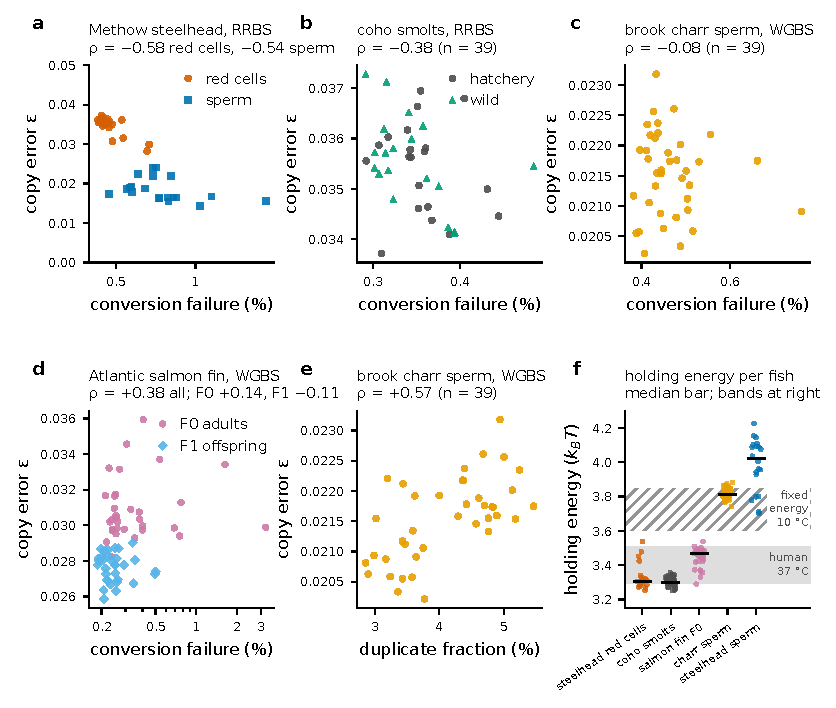
\includegraphics[width=\textwidth]{figures/part4/fig_fish_library.pdf}
\caption[Per-fish copy error against the library terms]{Per-fish copy error against the library terms. (a)--(d) Copy error against bisulfite conversion failure in each set; (e)
brook charr copy error against duplicate fraction; Spearman $\rho$ above each panel. Brook charr panels omit the failed download
(39 fish). Coho copy error as scored, without the sequencing-error subtraction. (f) Holding energy per fish
with the median as a bar; grey band, healthy human cells on the same statistic at 37~\textdegree C ($3.29$--$3.51\,\kB T$);
hatched band, the same energy held fixed in joules and read at 10~\textdegree C ($3.60$--$3.85\,\kB T$). All values are read
from the per-fish tables by the figure script. \measured{} for the readings; \calc{} for the hatched band.}
\label{fig:fishlibrary}
\end{figure}

\paragraph{The instrument repeats.} In every set the two halves of one fish agree, with ICC from 0.83 (coho, where the spread
between fish is smallest) to 0.998 (Table~\ref{tab:fishsets}). \measured

\paragraph{The fish do not yet show.} In every set the small spread between fish follows a library-quality term: conversion
failure in steelhead, coho and Atlantic salmon, duplicate fraction in brook charr (Figure~\ref{fig:fishlibrary}). The sign is not
the same in every set: negative in the two RRBS sets, positive in the Atlantic salmon fin. A per-read filter for incomplete conversion did not remove it. So no fish-level result exists: no hatchery
against wild difference, no line effect, no temperature effect and no individual trait has been read. \measured{} for the
correlations; the absence of a fish-level result is the outcome of the guards fixed in advance.

\paragraph{The holding energy.} Steelhead red cells (3.31), coho smolts (3.30, as scored) and Atlantic salmon fin (3.47~$\kB T$) read inside the range of healthy human cells on the same statistic,
$3.29$--$3.51\,\kB T$, and below the $3.60$--$3.85\,\kB T$ a holding energy fixed in joules would give at 10~\textdegree C.
Sperm read higher: $3.82\,\kB T$ in brook charr and $4.02\,\kB T$ in steelhead. \measured{} Read at face value, the fish keep
their copy error at about the same value in units of $\kB T$ as human cells, as if the holding energy scaled with temperature.
\interp{} This comparison is not the test. The fish and human values come from different library types and read pipelines,
and the copy error depends on the pipeline (Chapter~\ref{ch:iama}): ENCODE human blood cells, one donor per cell type, read
$3.76$--$3.93\,\kB T$ on the same statistic, higher than the human range above. RRBS reads CpG-dense regions, not the whole
genome. No fish in these sets has a recorded body temperature; 10~\textdegree C is the temperature assumed for the Methow water.
The temperature behaviour of the floor remains \openprob{} (Chapter~\ref{ch:temperature}).

\section{What the next fish set must have}

Two further public coho sets are downloaded and not yet read: a whole-genome bisulfite set (BioProject PRJNA641939) and a
reduced-representation set (BioProject PRJNA937312). \openprob

Each requirement answers a failure above.
\begin{enumerate}
\item \textbf{Whole-genome libraries with unique molecular identifiers.} WGBS or enzymatic methyl sequencing
      (EM-seq)~\cite{Vaisvila2021}, with a unique molecular identifier on every molecule~\cite{Kivioja2012}, so that duplicates are
      removed by molecule rather than by position. RRBS cannot be deduplicated, and the brook charr reading followed its duplicate
      fraction even after position-based deduplication.
\item \textbf{A known-pattern control in every library.} A spike-in of DNA whose methylation is known, unmethylated to read
      conversion and fully methylated to read the apparent copy error the library alone produces, so that each fish's copy error
      is read against what its own library does to a known pattern. The coho run showed that the library term is a property of the
      whole library, not of individual molecules, so it has to be measured per library.
\item \textbf{A per-fish temperature history.} A logged water temperature for the weeks before sampling, with sex, age and origin
      for every fish in the metadata. The Methow age check could not be run because age was not public, and no set so far has a
      recorded body temperature.
\item \textbf{One species, one cell type, two recorded temperatures, one pipeline.} Nucleated red cells from fish reared at two
      logged temperatures, read on the pipeline used for human cells. At $3.31\,\kB T$ and 10~\textdegree C, a holding energy fixed
      in joules raises the copy error by about 2~\% for $+2$~K and about 6~\% for $+5$~K; a value fixed in $\kB T$ leaves it
      unchanged. \calc{} The brook charr interval (0.79--1.05) shows how many fish such a test needs: the interval on the ratio must
      be narrower than the effect.
\end{enumerate}
The guard stays as it is: a correlation of $|\rho|\ge0.30$ with any library term, after the per-library control, blocks every
group comparison.

\begin{keybox}[title=What the fish showed]
The single-molecule copy error repeats within one fish in every set (ICC 0.83--0.998). Between fish it has so far followed a
library-quality term, conversion failure or duplication, so no fish-level, hatchery or wild, line or temperature result exists.
\measured{} The holding energy reads about $3.3\,\kB T$ in steelhead red cells and coho smolts at river temperature, as in human
cells at 37~\textdegree C, on different pipelines and without recorded body temperatures. \measured{} Whether the floor follows
temperature is \openprob{} until one species is read at two recorded temperatures on libraries with molecular identifiers and a
per-library known-pattern control.
\end{keybox}
